\documentclass[conf]{new-aiaa}
%\documentclass[12pt]{article}
% \usepackage[parfill]{parskip} % skip line instead of indenting paragraph
\usepackage[margin=1in]{geometry} % set margins
\usepackage{mathptmx} % Times New Roman
\usepackage{amsmath} % equations
\usepackage{graphicx} % figures
\usepackage{hyperref} % colored links
\usepackage{xcolor}  % colored text
\usepackage{titlesec} % custom section headings
\usepackage[breakable]{tcolorbox} % boxed text
\usepackage{enumitem} % custom lists
\usepackage{xurl} % allows line breaks un urls
\usepackage{listings} % list code
\usepackage{fancyvrb} % fancy verbatim code

\definecolor{psublue}{RGB}{0,51,175}
\definecolor{navy}{RGB}{23, 42, 86}
\definecolor{green}{RGB}{34,139,34}
\definecolor{red}{RGB}{210,0,0}
\definecolor{codegray}{gray}{0.5}
\definecolor{commentTeal}{RGB}{65, 128, 128}
\definecolor{cellborder}{RGB}{207,207,207}
\definecolor{cellbackground}{HTML}{F7F7F7}

\hypersetup{colorlinks=true, linkcolor=psublue, urlcolor = navy, citecolor=navy}

\newcommand{\Matlab}{\textsc{Matlab} } % make small caps MATLAB
\newcommand{\code}[1]{\colorbox{lightgray}{\texttt{#1}}} % format code function highlighted and monospace
\newcommand{\mat}[1]{\mathbf{#1}} % format math bold face

\lstdefinestyle{mystyle}{
    %backgroundcolor=\color{backcolour},   
    commentstyle=\color{commentTeal},
    keywordstyle=\color{green},
    numberstyle=\tiny\color{codegray},
    stringstyle=\color{red},
    basicstyle=\ttfamily\footnotesize,
	showstringspaces=false,
	numbers=left,
	breaklines=true
}
\lstset{style=mystyle}


\title{Autonomous UAV Navigation Using Reinforcement Learning}

\author{Kaosi Anyanwu and Kelly Harnish }
\affil{ ... }
\author{AERSP 597 - Machine Learning in Aerospace Engineering \\ Dr. Daning Huang}
\affil{Pennsylvania State University, State College, PA 16802}


\begin{document}
	
\maketitle

%%%%%%
\section{Background and Introduction}

Unmanned aerial vehicles (UAV) are used for missions in unknown environments that are too dangerous or difficult for humans. The major goal of a UAV is to operate and perform tasks autonomously without any human assistance. Over the last few years, UAV applications have grown to include delivery services and military use, involving navigating through hostile environments such as search and rescue missions, military operations, and wildfire monitoring. These applications have become extremely popular as the UAVs can hold numerous sensors to measure the environment at low operation costs and with high flexibility. Autonomous UAVs need to perceive and understand their environment to avoid collisions and have smooth flight and motion planning. It is difficult to implement this efficiently because data about the environment is normally limited or unavailable. To overcome this problem, reinforcement learning can be utilized as an approach to enhance UAV navigation. Reinforcement learning (RL) is a type of machine learning that takes suitable action to maximize reward for a particular situation. An RL agent does not know the best solution, rather the agent decides what next action to take based on a reward from previous actions, acting in a trial and error manner until it reaches the target, modeled simply in Figure \ref{fig:RLmodel}. Once the training environment is ready, the agent learns by itself rather than using a training data set. 

\begin{figure}[!htb]
	\centering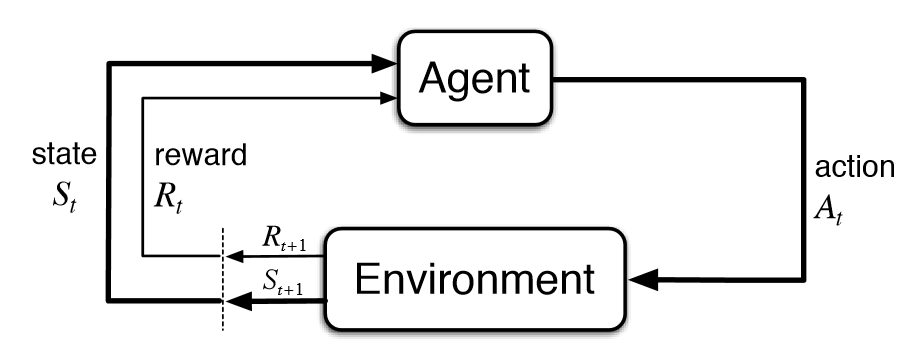
\includegraphics[width=4in]{RL_agent}
	\caption{\label{fig:RLmodel} Simple model of how an RL agent interacts with its environment}
\end{figure}


%%%%%%
\section{Methodology}

For this project, we will be utilizing Q-Learning. Q-Learning is a value-based RL algorithm that seeks to maximize its total reward. One challenge with real-life applications is that the states and actions are often continuous as opposed to discrete. In order to account for this in real-life applications, we will enhance the traditional RL algorithms by integrating deep learning neural networks to get a type deep reinforcement learning algorithm called deep Q-networks (DQN). We will DQNs to account for the sets of different states and actions. We will use Python to implement this algorithm on a drone modeled in a 2D environment first and then scale up to a 3D simulated environment, likely Unity. Python will utilize the TensorFlow library to carry out the DRL algorithm. OpenAI Gym will act as an interface to transfer image data and control actions from the 3D simulator to Python and vice versa. 


%%%%%%
\section{Conclusion}

The goal is to train a UAV to from the optimal path from a start point to target point while navigating in an unknown environment using a DQN. An interesting aspect would be to include sensors to avoid obstacles while doing this. 


%%%%%%
\nocite{Anwar2019}
\nocite{Araar2016}
\nocite{Carrio2017}
\nocite{Madaan}
\nocite{Pham2018}
\nocite{Rodriguez2018}
\nocite{Shin2019}

\bibliography{theBib}


%%%%%%%%
%\clearpage
%\section*{Code}

%\subsection*{Problem 1}
%\lstinputlisting[language=Python]{HW1_problem1.py}


\end{document}